\documentclass[1p]{elsarticle_modified}
%\bibliographystyle{elsarticle-num}

%\usepackage[colorlinks]{hyperref}
%\usepackage{abbrmath_seonhwa} %\Abb, \Ascr, \Acal ,\Abf, \Afrak
\usepackage{amsfonts}
\usepackage{amssymb}
\usepackage{amsmath}
\usepackage{amsthm}
\usepackage{scalefnt}
\usepackage{amsbsy}
\usepackage{kotex}
\usepackage{caption}
\usepackage{subfig}
\usepackage{color}
\usepackage{graphicx}
\usepackage{xcolor} %% white, black, red, green, blue, cyan, magenta, yellow
\usepackage{float}
\usepackage{setspace}
\usepackage{hyperref}

\usepackage{tikz}
\usetikzlibrary{arrows}

\usepackage{multirow}
\usepackage{array} % fixed length table
\usepackage{hhline}

%%%%%%%%%%%%%%%%%%%%%
\makeatletter
\renewcommand*\env@matrix[1][\arraystretch]{%
	\edef\arraystretch{#1}%
	\hskip -\arraycolsep
	\let\@ifnextchar\new@ifnextchar
	\array{*\c@MaxMatrixCols c}}
\makeatother %https://tex.stackexchange.com/questions/14071/how-can-i-increase-the-line-spacing-in-a-matrix
%%%%%%%%%%%%%%%

\usepackage[normalem]{ulem}

\newcommand{\msout}[1]{\ifmmode\text{\sout{\ensuremath{#1}}}\else\sout{#1}\fi}
%SOURCE: \msout is \stkout macro in https://tex.stackexchange.com/questions/20609/strikeout-in-math-mode

\newcommand{\cancel}[1]{
	\ifmmode
	{\color{red}\msout{#1}}
	\else
	{\color{red}\sout{#1}}
	\fi
}

\newcommand{\add}[1]{
	{\color{blue}\uwave{#1}}
}

\newcommand{\replace}[2]{
	\ifmmode
	{\color{red}\msout{#1}}{\color{blue}\uwave{#2}}
	\else
	{\color{red}\sout{#1}}{\color{blue}\uwave{#2}}
	\fi
}

\newcommand{\Sol}{\mathcal{S}} %segment
\newcommand{\D}{D} %diagram
\newcommand{\A}{\mathcal{A}} %arc


%%%%%%%%%%%%%%%%%%%%%%%%%%%%%5 test

\def\sl{\operatorname{\textup{SL}}(2,\Cbb)}
\def\psl{\operatorname{\textup{PSL}}(2,\Cbb)}
\def\quan{\mkern 1mu \triangleright \mkern 1mu}

\theoremstyle{definition}
\newtheorem{thm}{Theorem}[section]
\newtheorem{prop}[thm]{Proposition}
\newtheorem{lem}[thm]{Lemma}
\newtheorem{ques}[thm]{Question}
\newtheorem{cor}[thm]{Corollary}
\newtheorem{defn}[thm]{Definition}
\newtheorem{exam}[thm]{Example}
\newtheorem{rmk}[thm]{Remark}
\newtheorem{alg}[thm]{Algorithm}

\newcommand{\I}{\sqrt{-1}}
\begin{document}

%\begin{frontmatter}
%
%\title{Boundary parabolic representations of knots up to 8 crossings}
%
%%% Group authors per affiliation:
%\author{Yunhi Cho} 
%\address{Department of Mathematics, University of Seoul, Seoul, Korea}
%\ead{yhcho@uos.ac.kr}
%
%
%\author{Seonhwa Kim} %\fnref{s_kim}}
%\address{Center for Geometry and Physics, Institute for Basic Science, Pohang, 37673, Korea}
%\ead{ryeona17@ibs.re.kr}
%
%\author{Hyuk Kim}
%\address{Department of Mathematical Sciences, Seoul National University, Seoul 08826, Korea}
%\ead{hyukkim@snu.ac.kr}
%
%\author{Seokbeom Yoon}
%\address{Department of Mathematical Sciences, Seoul National University, Seoul, 08826,  Korea}
%\ead{sbyoon15@snu.ac.kr}
%
%\begin{abstract}
%We find all boundary parabolic representation of knots up to 8 crossings.
%
%\end{abstract}
%\begin{keyword}
%    \MSC[2010] 57M25 
%\end{keyword}
%
%\end{frontmatter}

%\linenumbers
%\tableofcontents
%
\newcommand\colored[1]{\textcolor{white}{\rule[-0.35ex]{0.8em}{1.4ex}}\kern-0.8em\color{red} #1}%
%\newcommand\colored[1]{\textcolor{white}{ #1}\kern-2.17ex	\textcolor{white}{ #1}\kern-1.81ex	\textcolor{white}{ #1}\kern-2.15ex\color{red}#1	}

{\Large $\underline{11a_{240}~(K11a_{240})}$}

\setlength{\tabcolsep}{10pt}
\renewcommand{\arraystretch}{1.6}
\vspace{1cm}\begin{tabular}{m{100pt}>{\centering\arraybackslash}m{274pt}}
\multirow{5}{120pt}{
	\centering
	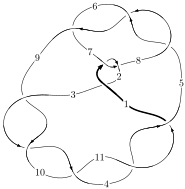
\includegraphics[width=112pt]{../../../GIT/diagram.site/Diagrams/png/489_11a_240.png}\\
\ \ \ A knot diagram\footnotemark}&
\allowdisplaybreaks
\textbf{Linearized knot diagam} \\
\cline{2-2}
 &
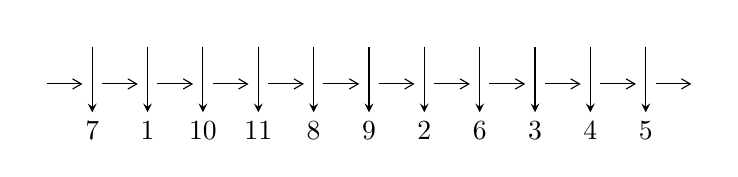
\begin{tikzpicture}[x=20pt, y=17pt]
	% nodes
	\node (C0) at (0, 0) {};
	\node (C1) at (1, 0) {};
	\node (C1U) at (1, +1) {};
	\node (C1D) at (1, -1) {7};

	\node (C2) at (2, 0) {};
	\node (C2U) at (2, +1) {};
	\node (C2D) at (2, -1) {1};

	\node (C3) at (3, 0) {};
	\node (C3U) at (3, +1) {};
	\node (C3D) at (3, -1) {10};

	\node (C4) at (4, 0) {};
	\node (C4U) at (4, +1) {};
	\node (C4D) at (4, -1) {11};

	\node (C5) at (5, 0) {};
	\node (C5U) at (5, +1) {};
	\node (C5D) at (5, -1) {8};

	\node (C6) at (6, 0) {};
	\node (C6U) at (6, +1) {};
	\node (C6D) at (6, -1) {9};

	\node (C7) at (7, 0) {};
	\node (C7U) at (7, +1) {};
	\node (C7D) at (7, -1) {2};

	\node (C8) at (8, 0) {};
	\node (C8U) at (8, +1) {};
	\node (C8D) at (8, -1) {6};

	\node (C9) at (9, 0) {};
	\node (C9U) at (9, +1) {};
	\node (C9D) at (9, -1) {3};

	\node (C10) at (10, 0) {};
	\node (C10U) at (10, +1) {};
	\node (C10D) at (10, -1) {4};

	\node (C11) at (11, 0) {};
	\node (C11U) at (11, +1) {};
	\node (C11D) at (11, -1) {5};
	\node (C12) at (12, 0) {};

	% arrows
	\draw[->,>={angle 60}]
	(C0) edge (C1) (C1) edge (C2) (C2) edge (C3) (C3) edge (C4) (C4) edge (C5) (C5) edge (C6) (C6) edge (C7) (C7) edge (C8) (C8) edge (C9) (C9) edge (C10) (C10) edge (C11) (C11) edge (C12) ;	\draw[->,>=stealth]
	(C1U) edge (C1D) (C2U) edge (C2D) (C3U) edge (C3D) (C4U) edge (C4D) (C5U) edge (C5D) (C6U) edge (C6D) (C7U) edge (C7D) (C8U) edge (C8D) (C9U) edge (C9D) (C10U) edge (C10D) (C11U) edge (C11D) ;
	\end{tikzpicture} \\
\hhline{~~} \\& 
\textbf{Solving Sequence} \\ \cline{2-2} 
 &
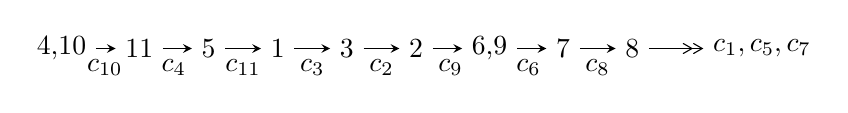
\begin{tikzpicture}[x=25pt, y=7pt]
	% node
	\node (A0) at (-1/8, 0) {4,10};
	\node (A1) at (1, 0) {11};
	\node (A2) at (2, 0) {5};
	\node (A3) at (3, 0) {1};
	\node (A4) at (4, 0) {3};
	\node (A5) at (5, 0) {2};
	\node (A6) at (97/16, 0) {6,9};
	\node (A7) at (57/8, 0) {7};
	\node (A8) at (65/8, 0) {8};
	\node (C1) at (1/2, -1) {$c_{10}$};
	\node (C2) at (3/2, -1) {$c_{4}$};
	\node (C3) at (5/2, -1) {$c_{11}$};
	\node (C4) at (7/2, -1) {$c_{3}$};
	\node (C5) at (9/2, -1) {$c_{2}$};
	\node (C6) at (11/2, -1) {$c_{9}$};
	\node (C7) at (53/8, -1) {$c_{6}$};
	\node (C8) at (61/8, -1) {$c_{8}$};
	\node (A9) at (10, 0) {$c_{1},c_{5},c_{7}$};

	% edge
	\draw[->,>=stealth]	
	(A0) edge (A1) (A1) edge (A2) (A2) edge (A3) (A3) edge (A4) (A4) edge (A5) (A5) edge (A6) (A6) edge (A7) (A7) edge (A8) ;
	\draw[->>,>={angle 60}]	
	(A8) edge (A9);
\end{tikzpicture} \\ 

\end{tabular} \\

\footnotetext{
The image of knot diagram is generated by the software ``\textbf{Draw programme}" developed by Andrew Bartholomew(\url{http://www.layer8.co.uk/maths/draw/index.htm\#Running-draw}), where we modified some parts for our purpose(\url{https://github.com/CATsTAILs/LinksPainter}).
}\phantom \\ \newline 
\centering \textbf{Ideals for irreducible components\footnotemark of $X_{\text{par}}$} 
 
\begin{align*}
I^u_{1}&=\langle 
- u^{31}+u^{30}+\cdots+b- u,\;- u^{31}+u^{30}+\cdots+a+1,\;u^{32}-2 u^{31}+\cdots-4 u+1\rangle \\
I^u_{2}&=\langle 
b+u,\;a+u+1,\;u^2+u-1\rangle \\
\\
\end{align*}
\raggedright * 2 irreducible components of $\dim_{\mathbb{C}}=0$, with total 34 representations.\\
\footnotetext{All coefficients of polynomials are rational numbers. But the coefficients are sometimes approximated in decimal forms when there is not enough margin.}
\newpage
\renewcommand{\arraystretch}{1}
\centering \section*{I. $I^u_{1}= \langle - u^{31}+u^{30}+\cdots+b- u,\;- u^{31}+u^{30}+\cdots+a+1,\;u^{32}-2 u^{31}+\cdots-4 u+1 \rangle$}
\flushleft \textbf{(i) Arc colorings}\\
\begin{tabular}{m{7pt} m{180pt} m{7pt} m{180pt} }
\flushright $a_{4}=$&$\begin{pmatrix}0\\u\end{pmatrix}$ \\
\flushright $a_{10}=$&$\begin{pmatrix}1\\0\end{pmatrix}$ \\
\flushright $a_{11}=$&$\begin{pmatrix}1\\u^2\end{pmatrix}$ \\
\flushright $a_{5}=$&$\begin{pmatrix}- u\\- u^3+u\end{pmatrix}$ \\
\flushright $a_{1}=$&$\begin{pmatrix}- u^2+1\\- u^4+2 u^2\end{pmatrix}$ \\
\flushright $a_{3}=$&$\begin{pmatrix}u\\u\end{pmatrix}$ \\
\flushright $a_{2}=$&$\begin{pmatrix}- u^7+4 u^5-4 u^3+2 u\\- u^9+5 u^7-7 u^5+2 u^3+u\end{pmatrix}$ \\
\flushright $a_{6}=$&$\begin{pmatrix}u^{31}- u^{30}+\cdots+3 u-1\\u^{31}- u^{30}+\cdots- u^2+u\end{pmatrix}$ \\
\flushright $a_{9}=$&$\begin{pmatrix}- u^2+1\\- u^2\end{pmatrix}$ \\
\flushright $a_{7}=$&$\begin{pmatrix}2 u^{31}- u^{30}+\cdots+5 u-2\\3 u^{31}-2 u^{30}+\cdots+4 u-1\end{pmatrix}$ \\
\flushright $a_{8}=$&$\begin{pmatrix}u^{30}- u^{29}+\cdots- u+1\\u^{31}-20 u^{29}+\cdots+3 u-1\end{pmatrix}$\\ \flushright $a_{8}=$&$\begin{pmatrix}u^{30}- u^{29}+\cdots- u+1\\u^{31}-20 u^{29}+\cdots+3 u-1\end{pmatrix}$\\&\end{tabular}
\flushleft \textbf{(ii) Obstruction class $= -1$}\\~\\
\flushleft \textbf{(iii) Cusp Shapes $= 4 u^{31}-5 u^{30}-77 u^{29}+93 u^{28}+654 u^{27}-766 u^{26}-3221 u^{25}+3695 u^{24}+10154 u^{23}-11648 u^{22}-21262 u^{21}+25364 u^{20}+29394 u^{19}-39216 u^{18}-24813 u^{17}+43171 u^{16}+8234 u^{15}-32696 u^{14}+6950 u^{13}+15056 u^{12}-10454 u^{11}-2100 u^{10}+5696 u^9-1812 u^8-1168 u^7+978 u^6-182 u^5-72 u^4+86 u^3-38 u^2+13 u-19$}\\~\\
\newpage\renewcommand{\arraystretch}{1}
\flushleft \textbf{(iv) u-Polynomials at the component}\newline \\
\begin{tabular}{m{50pt}|m{274pt}}
Crossings & \hspace{64pt}u-Polynomials at each crossing \\
\hline $$\begin{aligned}c_{1},c_{7}\end{aligned}$$&$\begin{aligned}
&u^{32}+u^{31}+\cdots-12 u-4
\end{aligned}$\\
\hline $$\begin{aligned}c_{2}\end{aligned}$$&$\begin{aligned}
&u^{32}+15 u^{31}+\cdots+152 u+16
\end{aligned}$\\
\hline $$\begin{aligned}c_{3},c_{4},c_{9}\\c_{10},c_{11}\end{aligned}$$&$\begin{aligned}
&u^{32}+2 u^{31}+\cdots+4 u+1
\end{aligned}$\\
\hline $$\begin{aligned}c_{5},c_{6},c_{8}\end{aligned}$$&$\begin{aligned}
&u^{32}-3 u^{31}+\cdots-5 u-1
\end{aligned}$\\
\hline
\end{tabular}\\~\\
\newpage\renewcommand{\arraystretch}{1}
\flushleft \textbf{(v) Riley Polynomials at the component}\newline \\
\begin{tabular}{m{50pt}|m{274pt}}
Crossings & \hspace{64pt}Riley Polynomials at each crossing \\
\hline $$\begin{aligned}c_{1},c_{7}\end{aligned}$$&$\begin{aligned}
&y^{32}-15 y^{31}+\cdots-152 y+16
\end{aligned}$\\
\hline $$\begin{aligned}c_{2}\end{aligned}$$&$\begin{aligned}
&y^{32}+y^{31}+\cdots-2848 y+256
\end{aligned}$\\
\hline $$\begin{aligned}c_{3},c_{4},c_{9}\\c_{10},c_{11}\end{aligned}$$&$\begin{aligned}
&y^{32}-42 y^{31}+\cdots-4 y+1
\end{aligned}$\\
\hline $$\begin{aligned}c_{5},c_{6},c_{8}\end{aligned}$$&$\begin{aligned}
&y^{32}-29 y^{31}+\cdots-7 y+1
\end{aligned}$\\
\hline
\end{tabular}\\~\\
\newpage\flushleft \textbf{(vi) Complex Volumes and Cusp Shapes}
$$\begin{array}{c|c|c}  
\text{Solutions to }I^u_{1}& \I (\text{vol} + \sqrt{-1}CS) & \text{Cusp shape}\\
 \hline 
\begin{aligned}
u &= -0.932935 + 0.300495 I \\
a &= \phantom{-}0.221529 - 0.245031 I \\
b &= -0.566090 - 0.639414 I\end{aligned}
 & -2.01989 + 4.86523 I & -15.1954 - 6.8122 I \\ \hline\begin{aligned}
u &= -0.932935 - 0.300495 I \\
a &= \phantom{-}0.221529 + 0.245031 I \\
b &= -0.566090 + 0.639414 I\end{aligned}
 & -2.01989 - 4.86523 I & -15.1954 + 6.8122 I \\ \hline\begin{aligned}
u &= \phantom{-}0.946587 + 0.231196 I \\
a &= \phantom{-}0.96950 - 1.13998 I \\
b &= -1.46374 + 0.52554 I\end{aligned}
 & -4.86072 - 2.90543 I & -17.9793 + 3.5680 I \\ \hline\begin{aligned}
u &= \phantom{-}0.946587 - 0.231196 I \\
a &= \phantom{-}0.96950 + 1.13998 I \\
b &= -1.46374 - 0.52554 I\end{aligned}
 & -4.86072 + 2.90543 I & -17.9793 - 3.5680 I \\ \hline\begin{aligned}
u &= -0.994935 + 0.377573 I \\
a &= -0.478871 - 1.164710 I \\
b &= \phantom{-}1.158740 + 0.411567 I\end{aligned}
 & -7.38074 + 8.76774 I & -18.7396 - 7.0546 I \\ \hline\begin{aligned}
u &= -0.994935 - 0.377573 I \\
a &= -0.478871 + 1.164710 I \\
b &= \phantom{-}1.158740 - 0.411567 I\end{aligned}
 & -7.38074 - 8.76774 I & -18.7396 + 7.0546 I \\ \hline\begin{aligned}
u &= -0.910087 + 0.140122 I \\
a &= \phantom{-}0.945898 + 0.573430 I \\
b &= \phantom{-}0.426810 + 0.536403 I\end{aligned}
 & -3.85845 + 0.52237 I & -20.0729 - 1.6653 I \\ \hline\begin{aligned}
u &= -0.910087 - 0.140122 I \\
a &= \phantom{-}0.945898 - 0.573430 I \\
b &= \phantom{-}0.426810 - 0.536403 I\end{aligned}
 & -3.85845 - 0.52237 I & -20.0729 + 1.6653 I \\ \hline\begin{aligned}
u &= -1.21444\phantom{ +0.000000I} \\
a &= -0.504163\phantom{ +0.000000I} \\
b &= \phantom{-}1.45498\phantom{ +0.000000I}\end{aligned}
 & -11.2682\phantom{ +0.000000I} & -22.0990\phantom{ +0.000000I} \\ \hline\begin{aligned}
u &= \phantom{-}0.588921 + 0.485955 I \\
a &= -1.26657 + 1.04213 I \\
b &= -0.886632 + 0.309455 I\end{aligned}
 & -4.95979 + 1.69559 I & -17.9188 + 0.0178 I\\
 \hline 
 \end{array}$$\newpage$$\begin{array}{c|c|c}  
\text{Solutions to }I^u_{1}& \I (\text{vol} + \sqrt{-1}CS) & \text{Cusp shape}\\
 \hline 
\begin{aligned}
u &= \phantom{-}0.588921 - 0.485955 I \\
a &= -1.26657 - 1.04213 I \\
b &= -0.886632 - 0.309455 I\end{aligned}
 & -4.95979 - 1.69559 I & -17.9188 - 0.0178 I \\ \hline\begin{aligned}
u &= \phantom{-}0.718238 + 0.225952 I \\
a &= -0.459114 - 0.005471 I \\
b &= \phantom{-}0.496105 - 0.264918 I\end{aligned}
 & -0.558920 - 0.474938 I & -11.62959 + 1.27773 I \\ \hline\begin{aligned}
u &= \phantom{-}0.718238 - 0.225952 I \\
a &= -0.459114 + 0.005471 I \\
b &= \phantom{-}0.496105 + 0.264918 I\end{aligned}
 & -0.558920 + 0.474938 I & -11.62959 - 1.27773 I \\ \hline\begin{aligned}
u &= \phantom{-}0.187060 + 0.621355 I \\
a &= -0.85945 + 1.47486 I \\
b &= -1.011920 + 0.169007 I\end{aligned}
 & -3.74023 - 5.38912 I & -14.5723 + 5.7053 I \\ \hline\begin{aligned}
u &= \phantom{-}0.187060 - 0.621355 I \\
a &= -0.85945 - 1.47486 I \\
b &= -1.011920 - 0.169007 I\end{aligned}
 & -3.74023 + 5.38912 I & -14.5723 - 5.7053 I \\ \hline\begin{aligned}
u &= \phantom{-}0.109732 + 0.502858 I \\
a &= -0.133670 - 0.948522 I \\
b &= \phantom{-}0.000513 + 0.345169 I\end{aligned}
 & \phantom{-}1.17199 - 2.12258 I & -8.07273 + 5.17972 I \\ \hline\begin{aligned}
u &= \phantom{-}0.109732 - 0.502858 I \\
a &= -0.133670 + 0.948522 I \\
b &= \phantom{-}0.000513 - 0.345169 I\end{aligned}
 & \phantom{-}1.17199 + 2.12258 I & -8.07273 - 5.17972 I \\ \hline\begin{aligned}
u &= -1.53142\phantom{ +0.000000I} \\
a &= \phantom{-}0.299106\phantom{ +0.000000I} \\
b &= \phantom{-}1.47350\phantom{ +0.000000I}\end{aligned}
 & -11.6098\phantom{ +0.000000I} & -22.5450\phantom{ +0.000000I} \\ \hline\begin{aligned}
u &= -0.130280 + 0.363295 I \\
a &= \phantom{-}1.12950 + 2.35629 I \\
b &= \phantom{-}0.957149 + 0.120157 I\end{aligned}
 & -1.55433 + 0.80952 I & -9.54426 - 1.40879 I \\ \hline\begin{aligned}
u &= -0.130280 - 0.363295 I \\
a &= \phantom{-}1.12950 - 2.35629 I \\
b &= \phantom{-}0.957149 - 0.120157 I\end{aligned}
 & -1.55433 - 0.80952 I & -9.54426 + 1.40879 I\\
 \hline 
 \end{array}$$\newpage$$\begin{array}{c|c|c}  
\text{Solutions to }I^u_{1}& \I (\text{vol} + \sqrt{-1}CS) & \text{Cusp shape}\\
 \hline 
\begin{aligned}
u &= -1.65686 + 0.03953 I \\
a &= \phantom{-}1.168620 + 0.485339 I \\
b &= \phantom{-}1.98443 + 0.52843 I\end{aligned}
 & -8.99808 + 1.32195 I & \phantom{-0.000000 } 0 \\ \hline\begin{aligned}
u &= -1.65686 - 0.03953 I \\
a &= \phantom{-}1.168620 - 0.485339 I \\
b &= \phantom{-}1.98443 - 0.52843 I\end{aligned}
 & -8.99808 - 1.32195 I & \phantom{-0.000000 } 0 \\ \hline\begin{aligned}
u &= \phantom{-}0.322365\phantom{ +0.000000I} \\
a &= -0.569030\phantom{ +0.000000I} \\
b &= \phantom{-}0.332706\phantom{ +0.000000I}\end{aligned}
 & -0.607216\phantom{ +0.000000I} & -16.6590\phantom{ +0.000000I} \\ \hline\begin{aligned}
u &= \phantom{-}1.69979 + 0.04032 I \\
a &= -0.740305 - 0.450279 I \\
b &= -1.60526 - 0.31431 I\end{aligned}
 & -13.16730 - 1.26120 I & \phantom{-0.000000 } 0 \\ \hline\begin{aligned}
u &= \phantom{-}1.69979 - 0.04032 I \\
a &= -0.740305 + 0.450279 I \\
b &= -1.60526 + 0.31431 I\end{aligned}
 & -13.16730 + 1.26120 I & \phantom{-0.000000 } 0 \\ \hline\begin{aligned}
u &= \phantom{-}1.70039 + 0.07638 I \\
a &= -1.024980 + 0.658959 I \\
b &= -1.73315 + 0.64681 I\end{aligned}
 & -11.32620 - 6.33717 I & \phantom{-0.000000 } 0 \\ \hline\begin{aligned}
u &= \phantom{-}1.70039 - 0.07638 I \\
a &= -1.024980 - 0.658959 I \\
b &= -1.73315 - 0.64681 I\end{aligned}
 & -11.32620 + 6.33717 I & \phantom{-0.000000 } 0 \\ \hline\begin{aligned}
u &= -1.70563 + 0.05938 I \\
a &= -3.73701 - 1.61459 I \\
b &= -6.32266 - 2.62594 I\end{aligned}
 & -14.2827 + 4.0537 I & \phantom{-0.000000 } 0 \\ \hline\begin{aligned}
u &= -1.70563 - 0.05938 I \\
a &= -3.73701 + 1.61459 I \\
b &= -6.32266 + 2.62594 I\end{aligned}
 & -14.2827 - 4.0537 I & \phantom{-0.000000 } 0 \\ \hline\begin{aligned}
u &= \phantom{-}1.71578 + 0.10104 I \\
a &= \phantom{-}2.85853 - 1.60940 I \\
b &= \phantom{-}4.90243 - 2.63065 I\end{aligned}
 & -16.9357 - 10.6981 I & \phantom{-0.000000 } 0\\
 \hline 
 \end{array}$$\newpage$$\begin{array}{c|c|c}  
\text{Solutions to }I^u_{1}& \I (\text{vol} + \sqrt{-1}CS) & \text{Cusp shape}\\
 \hline 
\begin{aligned}
u &= \phantom{-}1.71578 - 0.10104 I \\
a &= \phantom{-}2.85853 + 1.60940 I \\
b &= \phantom{-}4.90243 + 2.63065 I\end{aligned}
 & -16.9357 + 10.6981 I & \phantom{-0.000000 } 0 \\ \hline\begin{aligned}
u &= \phantom{-}1.75198\phantom{ +0.000000I} \\
a &= \phantom{-}3.58689\phantom{ +0.000000I} \\
b &= \phantom{-}6.06538\phantom{ +0.000000I}\end{aligned}
 & \phantom{-}17.6150\phantom{ +0.000000I} & \phantom{-0.000000 } 0\\
 \hline 
 \end{array}$$\newpage\newpage\renewcommand{\arraystretch}{1}
\centering \section*{II. $I^u_{2}= \langle b+u,\;a+u+1,\;u^2+u-1 \rangle$}
\flushleft \textbf{(i) Arc colorings}\\
\begin{tabular}{m{7pt} m{180pt} m{7pt} m{180pt} }
\flushright $a_{4}=$&$\begin{pmatrix}0\\u\end{pmatrix}$ \\
\flushright $a_{10}=$&$\begin{pmatrix}1\\0\end{pmatrix}$ \\
\flushright $a_{11}=$&$\begin{pmatrix}1\\- u+1\end{pmatrix}$ \\
\flushright $a_{5}=$&$\begin{pmatrix}- u\\- u+1\end{pmatrix}$ \\
\flushright $a_{1}=$&$\begin{pmatrix}u\\u\end{pmatrix}$ \\
\flushright $a_{3}=$&$\begin{pmatrix}u\\u\end{pmatrix}$ \\
\flushright $a_{2}=$&$\begin{pmatrix}u\\u\end{pmatrix}$ \\
\flushright $a_{6}=$&$\begin{pmatrix}- u-1\\- u\end{pmatrix}$ \\
\flushright $a_{9}=$&$\begin{pmatrix}u\\u-1\end{pmatrix}$ \\
\flushright $a_{7}=$&$\begin{pmatrix}-1\\-1\end{pmatrix}$ \\
\flushright $a_{8}=$&$\begin{pmatrix}-1\\-1\end{pmatrix}$\\ \flushright $a_{8}=$&$\begin{pmatrix}-1\\-1\end{pmatrix}$\\&\end{tabular}
\flushleft \textbf{(ii) Obstruction class $= 1$}\\~\\
\flushleft \textbf{(iii) Cusp Shapes $= -15$}\\~\\
\newpage\renewcommand{\arraystretch}{1}
\flushleft \textbf{(iv) u-Polynomials at the component}\newline \\
\begin{tabular}{m{50pt}|m{274pt}}
Crossings & \hspace{64pt}u-Polynomials at each crossing \\
\hline $$\begin{aligned}c_{1},c_{2},c_{7}\end{aligned}$$&$\begin{aligned}
&u^2
\end{aligned}$\\
\hline $$\begin{aligned}c_{3},c_{4}\end{aligned}$$&$\begin{aligned}
&u^2- u-1
\end{aligned}$\\
\hline $$\begin{aligned}c_{5},c_{6}\end{aligned}$$&$\begin{aligned}
&(u-1)^2
\end{aligned}$\\
\hline $$\begin{aligned}c_{8}\end{aligned}$$&$\begin{aligned}
&(u+1)^2
\end{aligned}$\\
\hline $$\begin{aligned}c_{9},c_{10},c_{11}\end{aligned}$$&$\begin{aligned}
&u^2+u-1
\end{aligned}$\\
\hline
\end{tabular}\\~\\
\newpage\renewcommand{\arraystretch}{1}
\flushleft \textbf{(v) Riley Polynomials at the component}\newline \\
\begin{tabular}{m{50pt}|m{274pt}}
Crossings & \hspace{64pt}Riley Polynomials at each crossing \\
\hline $$\begin{aligned}c_{1},c_{2},c_{7}\end{aligned}$$&$\begin{aligned}
&y^2
\end{aligned}$\\
\hline $$\begin{aligned}c_{3},c_{4},c_{9}\\c_{10},c_{11}\end{aligned}$$&$\begin{aligned}
&y^2-3 y+1
\end{aligned}$\\
\hline $$\begin{aligned}c_{5},c_{6},c_{8}\end{aligned}$$&$\begin{aligned}
&(y-1)^2
\end{aligned}$\\
\hline
\end{tabular}\\~\\
\newpage\flushleft \textbf{(vi) Complex Volumes and Cusp Shapes}
$$\begin{array}{c|c|c}  
\text{Solutions to }I^u_{2}& \I (\text{vol} + \sqrt{-1}CS) & \text{Cusp shape}\\
 \hline 
\begin{aligned}
u &= \phantom{-}0.618034\phantom{ +0.000000I} \\
a &= -1.61803\phantom{ +0.000000I} \\
b &= -0.618034\phantom{ +0.000000I}\end{aligned}
 & -2.63189\phantom{ +0.000000I} & -15.0000\phantom{ +0.000000I} \\ \hline\begin{aligned}
u &= -1.61803\phantom{ +0.000000I} \\
a &= \phantom{-}0.618034\phantom{ +0.000000I} \\
b &= \phantom{-}1.61803\phantom{ +0.000000I}\end{aligned}
 & -10.5276\phantom{ +0.000000I} & -15.0000\phantom{ +0.000000I}\\
 \hline 
 \end{array}$$\newpage
\newpage\renewcommand{\arraystretch}{1}
\centering \section*{ III. u-Polynomials}
\begin{tabular}{m{50pt}|m{274pt}}
Crossings & \hspace{64pt}u-Polynomials at each crossing \\
\hline $$\begin{aligned}c_{1},c_{7}\end{aligned}$$&$\begin{aligned}
&u^2(u^{32}+u^{31}+\cdots-12 u-4)
\end{aligned}$\\
\hline $$\begin{aligned}c_{2}\end{aligned}$$&$\begin{aligned}
&u^2(u^{32}+15 u^{31}+\cdots+152 u+16)
\end{aligned}$\\
\hline $$\begin{aligned}c_{3},c_{4}\end{aligned}$$&$\begin{aligned}
&(u^2- u-1)(u^{32}+2 u^{31}+\cdots+4 u+1)
\end{aligned}$\\
\hline $$\begin{aligned}c_{5},c_{6}\end{aligned}$$&$\begin{aligned}
&((u-1)^2)(u^{32}-3 u^{31}+\cdots-5 u-1)
\end{aligned}$\\
\hline $$\begin{aligned}c_{8}\end{aligned}$$&$\begin{aligned}
&((u+1)^2)(u^{32}-3 u^{31}+\cdots-5 u-1)
\end{aligned}$\\
\hline $$\begin{aligned}c_{9},c_{10},c_{11}\end{aligned}$$&$\begin{aligned}
&(u^2+u-1)(u^{32}+2 u^{31}+\cdots+4 u+1)
\end{aligned}$\\
\hline
\end{tabular}\newpage\renewcommand{\arraystretch}{1}
\centering \section*{ IV. Riley Polynomials}
\begin{tabular}{m{50pt}|m{274pt}}
Crossings & \hspace{64pt}Riley Polynomials at each crossing \\
\hline $$\begin{aligned}c_{1},c_{7}\end{aligned}$$&$\begin{aligned}
&y^2(y^{32}-15 y^{31}+\cdots-152 y+16)
\end{aligned}$\\
\hline $$\begin{aligned}c_{2}\end{aligned}$$&$\begin{aligned}
&y^2(y^{32}+y^{31}+\cdots-2848 y+256)
\end{aligned}$\\
\hline $$\begin{aligned}c_{3},c_{4},c_{9}\\c_{10},c_{11}\end{aligned}$$&$\begin{aligned}
&(y^2-3 y+1)(y^{32}-42 y^{31}+\cdots-4 y+1)
\end{aligned}$\\
\hline $$\begin{aligned}c_{5},c_{6},c_{8}\end{aligned}$$&$\begin{aligned}
&((y-1)^2)(y^{32}-29 y^{31}+\cdots-7 y+1)
\end{aligned}$\\
\hline
\end{tabular}
\vskip 2pc
\end{document}